\section{Theorie}
\label{sec:Theorie}

In diesem Versuch ist das Licht als eine Welle zu erfassen, welche mit der elektrischen Feldstärke 

\begin{equation}
    E(x,t) = E_0 \cos(kx-\omega t - \delta)
\end{equation}

beschrieben werden kann. Dabei ist \(k\) die Wellenzahl, \(x\) der Ort, \(t\) die Zeit, \(\omega\) die Frequenz und \(\delta\) ein Phasenwinkel. Hier kann demnach ebenso davon ausgegangen werden, dass zwei miteinander interferierende Lichtwellen durch Superposition beschrieben werden. Was da allerdings einfacher gemessen werden kann, ist die Lichtintensität \(I\), welche proportional zum Betragsquadrat der elektrischen Feldstärke ist. Für die Intensität ergibt sich also bei einer Interferenz zweier Wellen mit \(E_0\):

%Wieso Plural? Wieso ist das alles gelb angestrichen?

\begin{equation}
    I_{ges} \propto 2(E_0)^2(1+\cos(\delta_2 - \delta_1))
\end{equation}

Der zweite Summand in der Klammer ist der Interferenzterm. Falls dieser Null wird, erreicht die Intensität ihr Maximum und falls dieser Term zu \(\pi\) wird, erreicht die Intensität ihr Minimum. Dies erfolgt weiterhin bei geraden Vielfachen von \(\pi\). Das Phänomen wird konstruktive- und destruktive Interferenz genannt, bei der sich die Amplituden einer Lichtwelle addieren, oder voneinander subtrahieren, sodass das Licht verschwindet. Dabei ist zu unterscheiden, ob diese Interferenzen örtlich bzw. zeitlich konstant aufrecht gehalten werden. Übliches Licht ist nicht kohärent, da die Wellen zeitlich statistisch verteilt sind. Kohärentes Licht, erzeugt mit Lasern beispielsweise, hat die Eigenschaft, dass die Phasendifferenz zweier Lichtwellen überall gleich bleibt. Bei einem Strahlenteiler wird deutlich, dass sich nicht immer Interferenzen beobachten lassen. 

%Vielfache von Pi ist doch klar... oder war das die Ausdrucksweise?

\begin{figure}
    \centering
    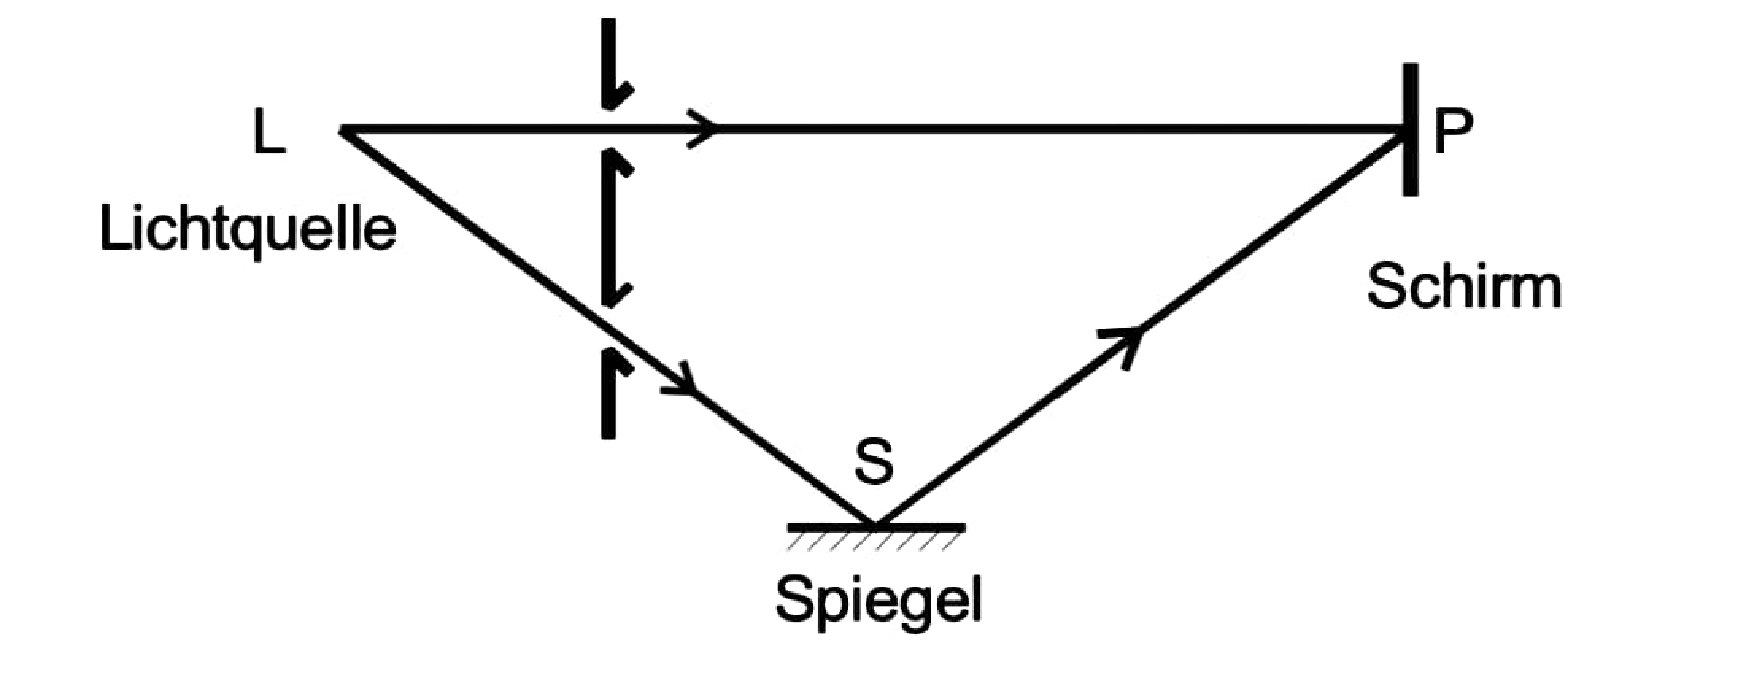
\includegraphics[scale = 0.3]{content/Strahlenteiler.pdf}
    \caption{Hier zu sehen ist eine Skizze zum besagten Strahlenteiler.}
    \label{fig:Teiler}
\end{figure}

Es können keine Interferenzen mehr auftreten, falls der Wegunterschied der Lichtstrahlen größer als die Länge der Lichtzüge, weil die Lichtstrahlen zu zwei verschiedenen Zeiten den Beobachtungspunkt P erreichen. Von diesem Punkt bis zum nächsten Punkt, an dem das Licht verschwindet, ist die Kohärenzlänge. Sie ist der Abstand zweier Maxima zueinander. Die Kohärenzlänge \(l\) wird definiert als

\begin{equation}
    l = N\lambda,
\end{equation}
wobei \(\lambda\) die Wellenlänge ist und \(N\) der Abstand zweier beobachteten Interferenzmaxima.
\\
Das Teilen des Lichtstrahls erfolgt dann mit dem Michaelson-Interferometer.

\begin{figure}
    \centering
    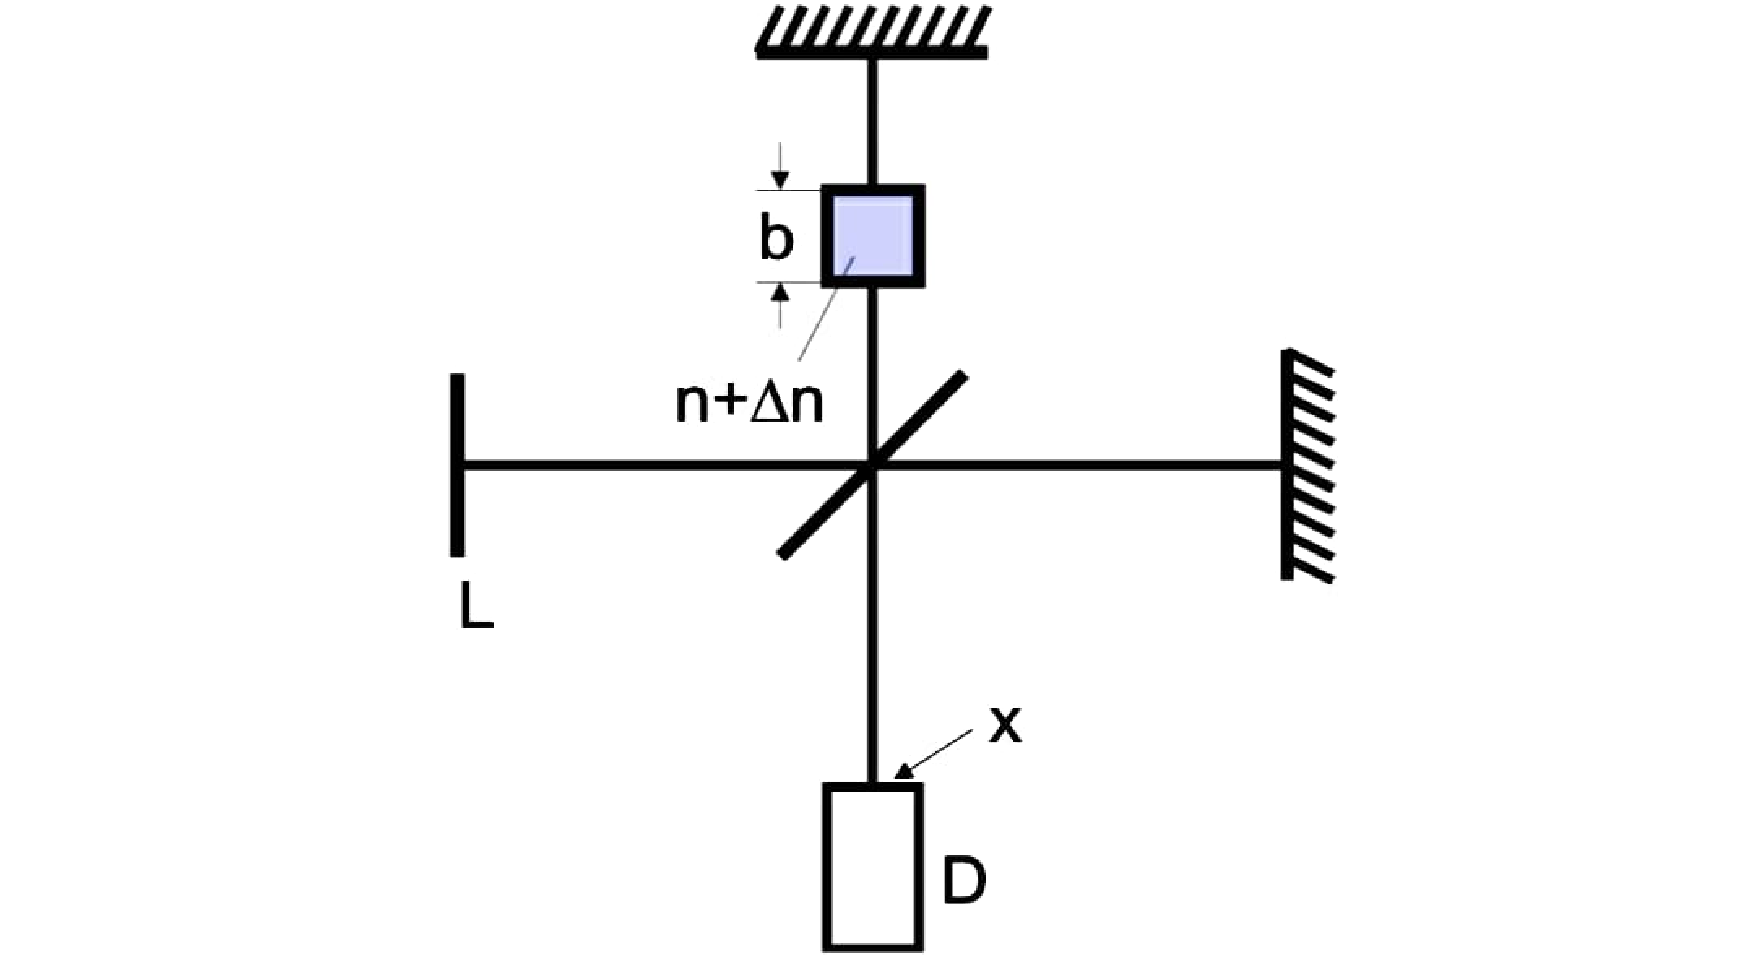
\includegraphics[scale = 0.3]{content/Interferometer.pdf}
    \caption{Hier zu sehen ist eine Skizze zum Interferometer.}
    \label{fig:Interferometer}
\end{figure}

Es werde, wie in \autoref{fig:Interferometer}, ein Strahl durch das Material laufen lassen, sodass es auf den Spiegel S2 trifft. Der andere Strahl wird auf S1 gerichtet. Dabei verläuft der Strahl durch kein Material. Beide Strahlen werden reflektiert und treffen in P aufeinander, wobei interferiert wird. Beide kommen hinterher auf den Detektor D zu. Beide Strahlen sind dementsprechend kohärent. Es gilt dabei dieser Zusammenhang zwischen der Verschiebung \(d\), die Anzahl der beobachteten Interferenzmaxima \(z\) und der Wellenlänge \(\lambda\):

\begin{equation}
   2d=z\lambda.
   \label{eq:verschiebung}
\end{equation}

Läuft ein Strahl dann durch ein Medium mit anderem Brechungsindex, so gilt mit der Änderung des Brechungsindex \(\Delta n\):

\begin{equation}
    2b\Delta n = z\lambda,
\end{equation}

wobei \(n\) durch eine Taylorentwicklung nach \(f(\lambda)\) angenähert werden kann:

\begin{equation}
    n = 1+\frac{f}{2} N
    \label{eq:pups}
\end{equation}

Mit 

\begin{equation}
    N(p,T) = \frac{pT_0}{p_0T} N_L
\end{equation}

und 

\begin{equation}
    \Delta n(p,p') = \frac{fT_0}{2p_0T} N_L (p-p')
\end{equation}

ergibt nicht nach Umstellung der \autoref{eq:pups} folgende Formel:

\begin{equation}
    n(p_0,T_0) = 1 + \frac{z\lambda T p_0}{2bT_0 (p-p')}.
    \label{eq:Druck}
\end{equation}